\documentclass[11pt]{article} 

% transcribed by Charles Zheng

% packages with special commands
\usepackage{amssymb, amsmath}
\usepackage{epsfig}
\usepackage{array}
\usepackage{ifthen}
\usepackage{color}
\usepackage{fancyhdr}
\usepackage{graphicx}
\usepackage{indentfirst}
\usepackage{caption}
%\usepackage{mathtools}
\definecolor{grey}{rgb}{0.5,0.5,0.5}

\begin{document}
\newcommand{\tr}{\text{tr}}
\newcommand{\E}{\textbf{E}}
\newcommand{\diag}{\text{diag}}
\newcommand{\argmax}{\text{argmax}}
\newcommand{\argmin}{\text{argmin}}
\newcommand{\Cov}{\text{Cov}}
\newcommand{\Vol}{\text{Vol}}
\pagestyle{fancy}

\title{Differential Geometric Theory of Statistics}

\author{Shun-ichi Amari\thanks{
Department of Mathematical Engineering and Instrumentation Physics, University of Tokyo, Tokyo, Japan}}

\maketitle

\tableofcontents

\section{Introduction}

       
            Statistics is a science which studies methods of inference, from
observed data, concerning the probabilistic structure underlying such data.
The class of all the possible probability distributions is usually too wide to
consider all its elements as candidates for the true probability distribution
from which the data were derived.  Statisticians often assume a statistical
model which is a subset of the set of all the possible probability distribut{ions,}
      and evaluate procedures of statistical inference assuming that the model
is faithful, i.e., it includes the true distribution.  It should, howver, be
remarked that a model is not necessarily faithful but is approximately so.  In
either case, it should be very important to know the shape of a statistical
model in the whole set of probability distributions.  This is the geometry of a
statistical model.  A statistical model often forms a geometrical manifold, so
that the geometry of manifolds should play an important role.  Considering that
properties of specific types of probability distributions, for example, of
Gaussian distributions, of Wiener processes, and so on, have so far been studied
in detail, it seems rather strange that only a few theories have been proposed
concerning properties of a family itself of distributions.  Here, by the proper{ties}
     of a family we mean such geometric relations as mutual distances, flatness
or curvature of the family, etc.  Obviously it is not a trivial task to define 
such geometric structures in a natural, useful and invariant manner.

            Only local properties of a statistical model are responsible for the
asymptotic theory of statistical inference.  Local properties are represented
by the geometry of the tangent spaces of the manifold.  The tangent space has a
natural Riemannian metric given by the Fisher information matrix in the regular
case.  It represents only a local property of the model, because the tangent
space is nothing but local linearization of the model manifold.  In order to
obtain larger-scale properties, one needs to define mutual relations of the two
different tangent spaces at two neighboring points in the model.  This can be
done by defining a one-to-one affine correspondence between two tangent spaces,
which is called an affine connection in differential geometry.  By an affine
connection, one can consider local properties around each point beyond the
linear approximation.  The curvature of a model can be obtained by the use of
this connection.  It is clear that such a differential-geometrical concept pro{vides}
      a tool convenient for studying higher-order asymptotic properties of
inference.  However, by connecting local tangent spaces further, one can obtain
global relations.  Hence, the validity of the differential-geometrical method is
not limited within the framework of asymptotic theory.

            It was Rao (1945) who first pointed out the importance in the
differential-geometrical approach.  He introduced the Riemannian metric by using
the Fisher information matrix.  Although a number of researches have been
carried out along this Riemannian line (see, e.g., Amari (1968), Atkinson and
Mitchell (1981), Dawid (1977), James (1973), Kass (1980), Skovgaard (1984),
Yoshizawa (1971), etc.), they did not have a large impact on statistics.  Some
additional concepts are necessary to improve its usefulness.  A new idea was
developed by Chentsov (1972) in his Russian book (and in some papers prior to
the book).  He introduced a family of affine connections and proved their unique{ness}
     from the point of view of categorical invariance.  Although his theory was
deep and fundamental, he did not discuss the curvature of a statistical model.
Efron (1975, 1978), independently of Chentsov's work, provided a new idea by 
pointing out that the statistical curvature plays an important role in higher-order
      properties of statistical inference.  Dawid (1975) pointed out further
possibilities.  Efron's idea was generalized by Madsen (1979) (see also Reeds
(1975)).  Amari (1980, 1982a) constructed a differential-geometrical method in
statistics by introducing a family of affine connections, which however turned
out to be equivalent to Chentsov's.  He further defined $\alpha$-curvatures, and pointed
   out the fundamental roles of the exponential and mixture curvatures played in
statistical inference.  The theory has been developed further by a number of
papers (Amari (1982b, 1983a, b), Amari and Kumon (1983), Kumon and Amari (1983,
1984, 1985), Nagaoka and Amari (1982), Eguchi (1983), Kass (1984)).  The new
developments were also shown in the NATO Research Workshop on Differential Geo{metry}
      in Statistical Inference (see Barndorff-Nielsen (1985) and Lauritzen
(1985)).  They together seem to prove the usefulness of differential geometry as
a fundamental method in statistics.  (See also Csisz\'{a}r (1975), Burbea and Rao
(1982), Pfanzagl (1982), Beale (1960), Bates and Watts (1980), etc., for other
geometrical work.)

            The present article gives not only a compact review of various
achievements up to now by the differential geometrical method most of which have
already been published in various journals and in Amari (1985) but also a pre{view}
     of new results and half-baked ideas in new directions, most of which have
not yet been published.  Chapter 2 provides an introduction to the geometrical
method, and elucidates fundamental geometrical properties of statistical mani{folds.}
        Chapter 3 is devoted to the higher-order asymptotic theory of statisti{cal}
    inference, summarizing higher-order characteristics of various estimators
and tests in geometrical terms.  Chapter 4 discusses a higher-order theory of
asymptotic sufficiency and ancillarity from the Fisher information point of
view.  Refer to Amari (1985) for more detailed explanation in these chapters;
Lauritzen (1985) gives a good introduction to modern differential geometry.  The
remaining Chapters 5, 6, and 7 treat new ideas and developments which are just
under construction.  In Chapter 5 is introduced a fibre bundle approach, which
is necessary in order to study properties of statistical inference in a general
statistical model other than a curved exponential family.  A Hilbert bundle and
a jet bundle are treated in a geometrical framework of statistical inference.
Chapter 6 gives a summary of a theory of estimation of a structural parameter
in the presence of nuisance parameters whose number increases in proportion to
the number of observations.  Here, the Hilbert bundle theory plays an essential
role.  Chapter 7 elucidates geometrical structures of parametric and non-para{metric}
       models of stationary Gaussian time series.  The present approach is use{ful}
    not only for constructing a higher-order theory of statistical inference on
time series models, but also for constructing differential geometrical theory of
systems and information theory (Amari, 1983 c).  These three chapters are
original and only sketches are given in the present paper.  More detailed theo{retical}
        treatments and their applications will appear as separate papers in the
near future.

\section{Geometrical Structure of Statistical Models}

\subsection{Metric and $\alpha$-connection}

Let $\mathcal{S} = \{p (x,\theta)\}$ be a statistical model consisting of probability
density functions $p(x, \theta)$ of random variable $x \in \mathcal{X}$ with respect to a measure $P$ on
$\mathcal{X}$ such that every distribution is uniquely parameterized by an $n$-dimensional
vector parameter $\theta = (\theta^i) = (\theta^1, \hdots, \theta^n)$.  Since the set $\{p(x)\}$ of all the
density functions is a subset of the $L_1$ space of functions in $x$, $\mathcal{S}$ is
considered to be a subset of the $L_1$ space.  A statistical model $\mathcal{S}$ is said to be
geometrically regular, when it satisfies the following regularity conditions
$\text{A}_1$ to $\text{A}_6$, and $S$ is regarded as an $n$-dimensional manifold with a coordinate system $\theta$.

\begin{description}
\item[$\text{A}_1$.] The domain $\Theta$ of the parameter $\theta$ is homeomorphic to an
$n$-dimensional Euclidean space $\mathbb{R}^n$
\item[$\text{A}_2$.] The topology of $\mathcal{S}$ induced from $\mathbb{R}^n$ is compatible with the
relative topology of $\mathcal{S}$ in $L_1$ space.
\item[$\text{A}_3$.] The support of $p(x, \theta)$ is common for all $\theta \in \Theta$, so that $p(x,\theta)$
are mutually absolutely continuous.
\item[$\text{A}_4$.] Every density function $p(x, \theta)$ is a smooth function in $\theta$ uniformly
in $x$, and the partial derivative $\frac{\partial}{\partial \theta^i}$ and the integration of $\log p(x, \theta)$
with respect to measure $P(x)$ are always commutative.
\item[$\text{A}_5$.] The moments of the score function $(\frac{\partial}{\partial \theta^i}) \log p(x, \theta)$ exist
up to the third order and are smooth in $\theta$.
\item[$\text{A}_6$.] The Fisher information matrix is positive definite.
\end{description}

Condition 1 implies that $\mathcal{S}$ itself is homeomorphic to $\mathbb{R}^n$.  It is
possible to weaken Condition 1.  However, only local properties are treated
here so that we assume it for the sake of simplicity.  In a later section, we
assume one more condition which guarantees the validity of Edgeworth expansions.

\begin{figure}[h]
\centering
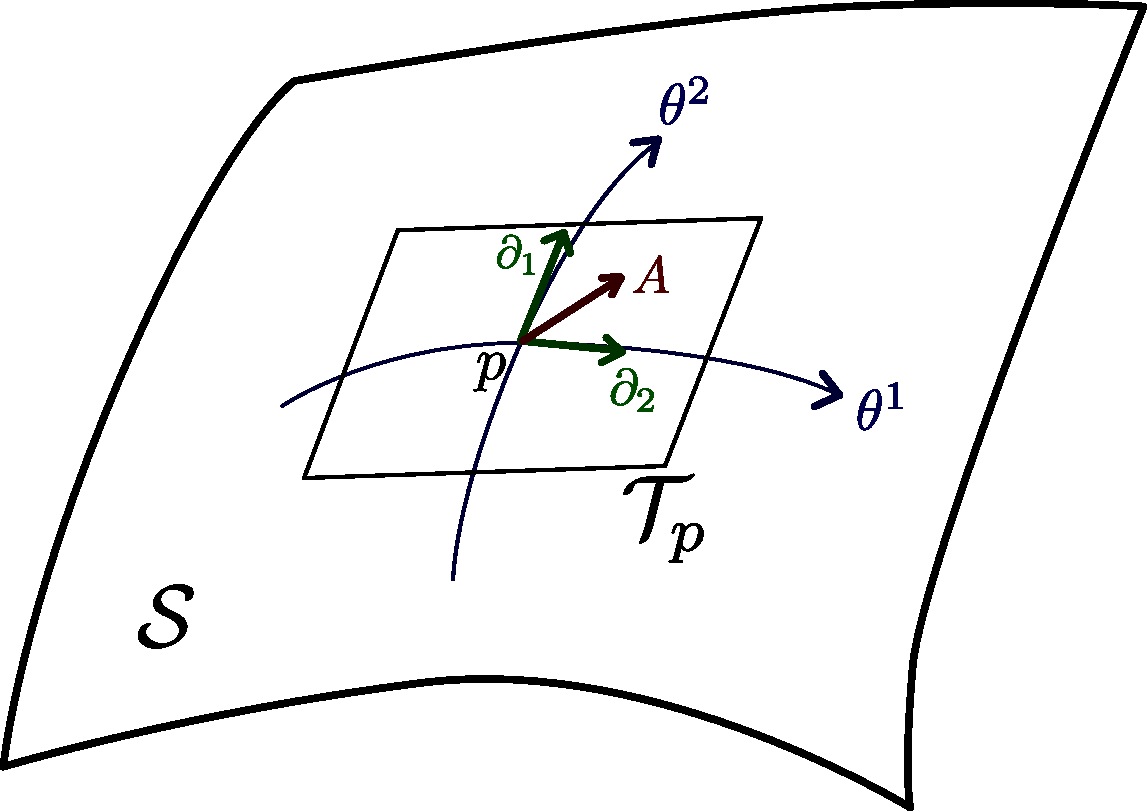
\includegraphics[scale = 0.3]{fig1.pdf}
\caption{}
\end{figure}

Let us denote by $\partial_i = \frac{\partial}{\partial \theta^i}$ the tangent vector $e_i$ of the $i$th
coordinate curve $\theta^i$ (Fig. 1) at point $\theta$.  Then, $n$ such tangent vectors $e_i = \partial_i$,
$i = 1, \hdots, n$, span the tangent space $\mathcal{T}_\theta$ at point $\theta$ of the manifold $\mathcal{S}$.
Any tangent vector $A \in \mathcal{T}_\theta$ is a linear combination of the basis vectors $\partial_i$,
\[
A = A^i \partial_i
\]
where $A^i$ are the components of vector $A$ and Einstein's sumamtion convection is
assumed throughout the paepr, so that the summation $\sum$ is automatically taken
for those indices which appear twice in one term once as a subscript and once as
a superscript.  The tangent space $\mathcal{T}_\theta$ is a linearized version of a small
neighborhood at $\theta$ of $\mathcal{S}$, and an infinitesimal vector $d\theta = d\theta^i \partial_i$ denotes the vector
connecting two neighboring points $\theta$ and $\theta + d\theta$ or two neighboring distributions
$p(x, \theta)$ and $p(x, \theta + d\theta)$.

Let us introduce a metric in the tangent space $\mathcal{T}_\theta$.
It can be done by defining the inner product $g_{ij}(\theta) = \langle
\partial_i, \partial_j \rangle$ of two basis vectors $\partial_i$ aand
$\partial_j$ at $\theta$.  To this end, we represent a vector
$\partial_i \in \mathcal{T}_\theta$ by a function $\partial_i \ell(x,
\theta)$ in $x$, where $\ell(x, \theta) = \log p(x, \theta)$ and
$\partial_i$ (in $\partial_i \ell$) is the partial derivative
$\frac{\partial}{\partial \theta^i}$.
Then, it is natural to define the inner product by
\begin{equation}
g_{ij}(\theta) = \langle \partial_i, \partial_j \rangle = 
\E_\theta[\partial_i \ell(x, \theta)\partial_j \ell(x,\theta)],\tag{2.1}\label{eq:2.1}
\end{equation}
where $\E_\theta$ denotes the expectation with respect to $p(x, \theta)$. This $g_{ij}$ is the
Fisher information matrix. Two vectors $A$ and $B$ are orthogonal when
\[
\langle A, B \rangle = \langle A^i \partial_i, B^j \partial_j \rangle = A^i B^j g_{ij} = 0.
\]

\section{Higher-Order Asymptotic Theory of Statistical Inference in Curved Exponential Family}

\section{Information, Sufficiency and Ancillarity Higher Order Theory}

\section{Fibre-Bundle Theory of Statistical Models}

\section{Estimation of Structural Parameter in the Presence of Infinitely Many Nuisance Parameters}

\section{Parametric Models of Stationary Gaussian Time Series}

\section{References}

\end{document}
